% Created 2020-04-12 日 12:13
% Intended LaTeX compiler: pdflatex
\documentclass[11pt]{article}
\usepackage[utf8]{inputenc}
\usepackage[T1]{fontenc}
\usepackage{graphicx}
\usepackage{grffile}
\usepackage{longtable}
\usepackage{wrapfig}
\usepackage{rotating}
\usepackage[normalem]{ulem}
\usepackage{amsmath}
\usepackage{textcomp}
\usepackage{amssymb}
\usepackage{capt-of}
\usepackage{hyperref}
\author{LZJ}
\date{\today}
\title{}
\hypersetup{
 pdfauthor={LZJ},
 pdftitle={},
 pdfkeywords={},
 pdfsubject={},
 pdfcreator={Emacs 26.3 (Org mode 9.4)}, 
 pdflang={English}}
\begin{document}

\begin{center}
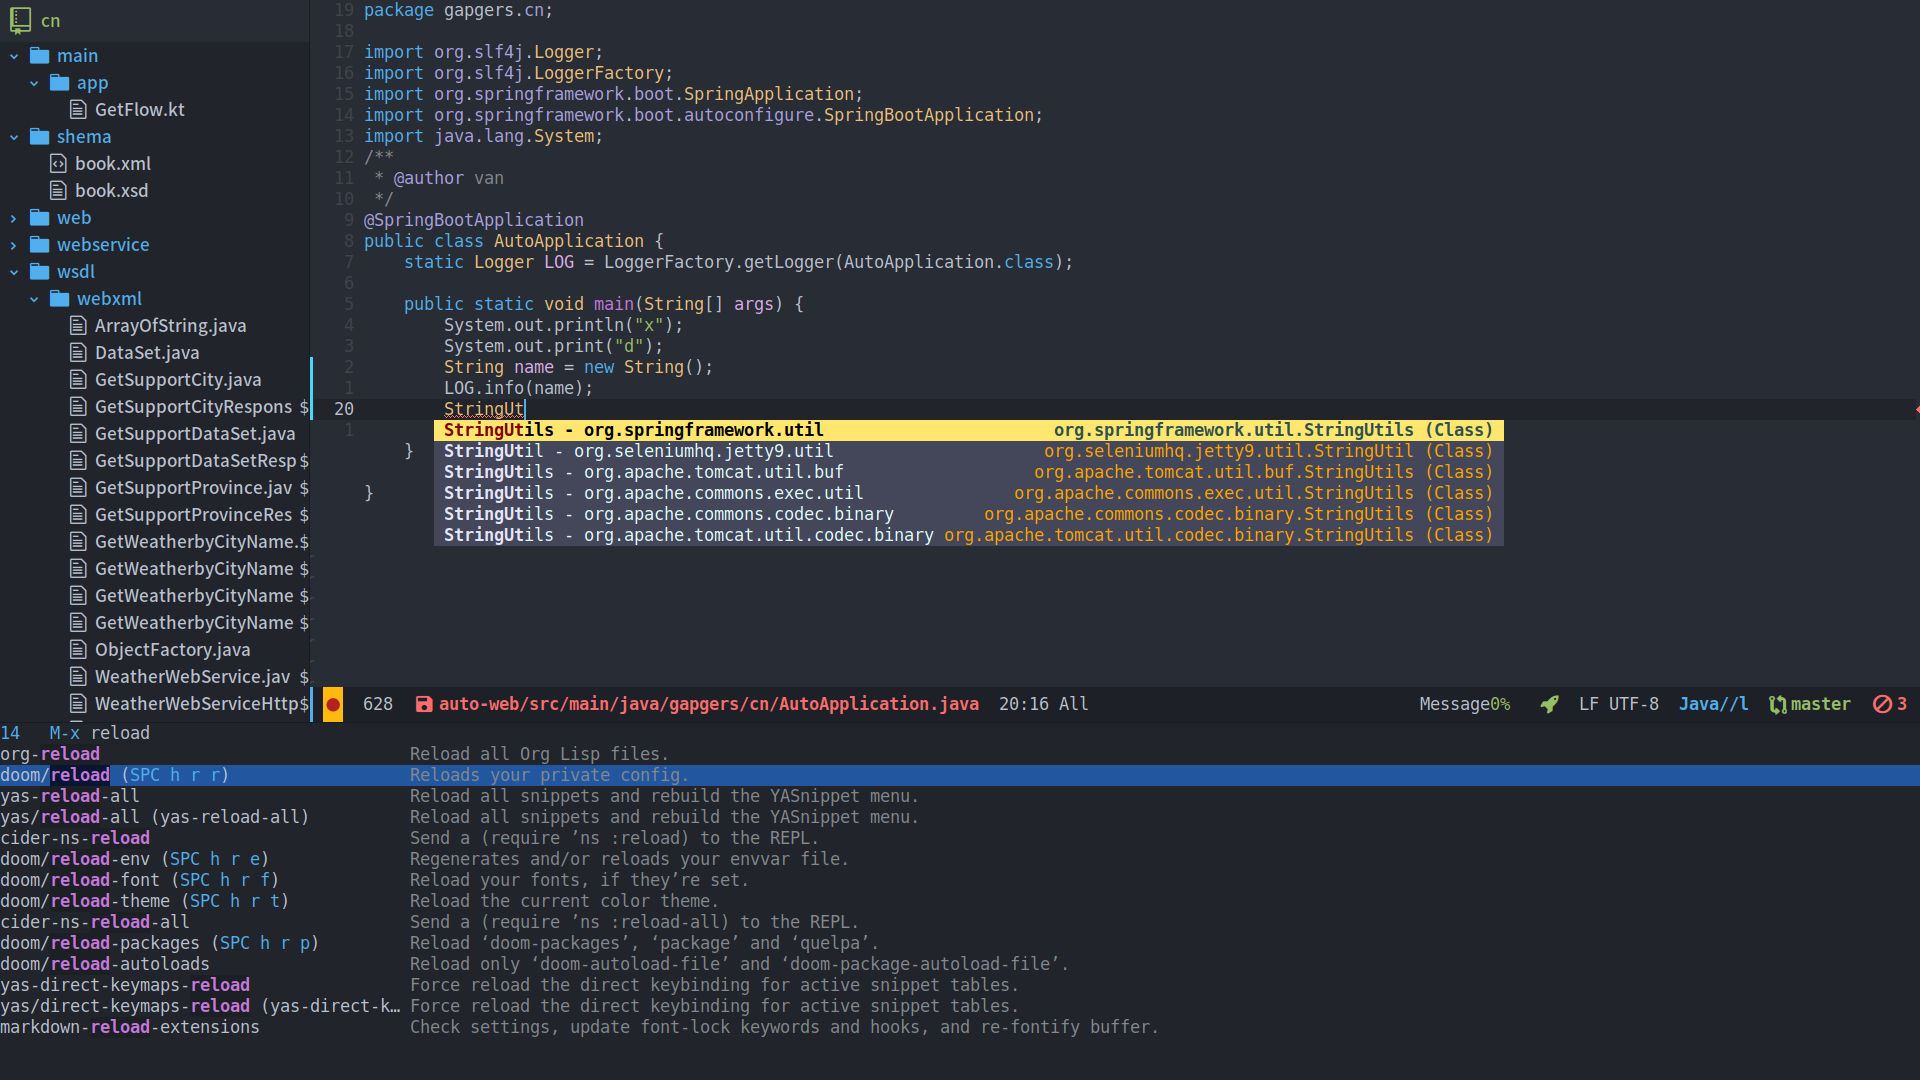
\includegraphics[width=.9\linewidth]{cut.png}
\end{center}

\section{PLUGINS \& FEATURES}
\label{sec:org3500d03}
\begin{enumerate}
\item lsp-java
\item ejc-sql
\item evil-fcitx
\item insert-translated-name
\item plantuml uml
\item number-region
\item counsel-fzf-dir-function
\item custom-set-faces
\item some shortcuts
\end{enumerate}
\section{INSTALL EMACS}
\label{sec:orgee666c2}
Choose your operation system and install it.

\url{https://www.gnu.org/software/emacs/}
\section{CLONE DOOM}
\label{sec:org0743b1e}

\begin{verbatim}
clone https://github.com/hlissner/doom-emacs.git ~/.emacs.doom/
\end{verbatim}
\section{CLONE REPOSITORY}
\label{sec:org259f84a}

\begin{verbatim}
git clone https://github.com/vanniuner/emacs-doom-private.git ~/.doom.d/
\end{verbatim}
\section{DOOM INSTALL}
\label{sec:org7674ed5}
Make sure that you have some setting in your terminal environment.

Set up a vpn if you need it.

\begin{verbatim}
export http_proxy="ip:port"
export https_proxy="ip:port"
\end{verbatim}

Set your emacs cmd for doom install.

\begin{verbatim}
export EMACS=/bin/emacs26
\end{verbatim}

At last run below, this will take few minutes. And it depends on the quality of your network.

\begin{verbatim}
~/.emacs.doom/bin/doom install
\end{verbatim}
\section{DEPENDENCIES}
\label{sec:org00914c0}

\url{https://github.com/junegunn/fzf}

\url{https://github.com/BurntSushi/ripgrep}

\url{https://github.com/kostafey/ejc-sql}

\url{https://plantuml.com/}

\url{https://github.com/emacs-lsp/lsp-java}
\end{document}
